\documentclass{article}

\usepackage[utf8]{inputenc}
\usepackage{geometry}
 \geometry{
 a4paper,
 total={170mm,257mm},
 left=20mm,
 top=20mm,
 }

% \usepackage[utf8]{inputenc}
% \usepackage{changepage}
% \usepackage[Sonny]{sty/fncychapleo}
\usepackage{mathptmx}  % times roman, including math (where possible)
\usepackage{palatino}  % palatino, including math (where possible)
\usepackage{helvet}    % helvetica
\usepackage{amsmath}
\usepackage{amssymb}
\usepackage{caption}

% \usepackage[square,sort,comma,numbers]{natbib}
% \usepackage{matrix}
\usepackage[compress, sort, numbers]{natbib}
\usepackage{mathtools}
\usepackage{nicefrac}
\usepackage{epigraph}
\usepackage{etoolbox}
\usepackage{xspace}
\usepackage{amsthm}
\usepackage{thmtools}
\usepackage{framed}
\usepackage{hhline}
\usepackage{graphicx}
\usepackage{graphbox}
\usepackage{pgfplots}
\usepackage{tikz}
\usepackage{fancybox}
\usepackage[T1]{fontenc}
\usepackage{pythonhighlight}
\usepackage{hyperref}
\usepackage{multicol}
\hypersetup{
     colorlinks   = true,
     citecolor    = blue
}

% ==============================================================
\newcommand{\vv}[1]{{\overrightarrow{#1}}}
\newcommand{\rasta}{\textit{\textsc{Ravestate}}\xspace}
\newcommand{\mathsc}[1]{\text{\textsc{#1}}}
\newenvironment{Figure}
  {\par\medskip\noindent\minipage{\linewidth}}
  {\endminipage\par\medskip}
   
\newtheorem{definition}{Definition}
\newtheorem{equ}{Equation}
\ignoretheorems{equ}

% ==============================================================
\title{Ravestate: Multimodal Contextual Dialog State Tracking As Bayesian Specific Signal Transduction}
\author{
	Birkner, Joseph \\ \texttt{joseph.birkner@tum.de}
	\and
	Karimi, Negin \\ \texttt{negin.karimi@tum.de}
	\and
	Hostettler, Rafael \\ \texttt{rh@gi.ai}
	\and
	Dolp, Andreas \\ \texttt{andreas.dolp@tum.de}
	\and
	Airiian, Wagram\\ \texttt{wagram.airiian@tum.de}
	\and
	Kharchenko, Alona \\ \texttt{unicorn@roboy.org}
}
\date{\vspace{-5ex}}

% ==============================================================
\begin{document}

\maketitle
\hrulefill

\begin{multicols}{2}

\section{Abstract}

A major challenge in the development of Natural Language Dialogue Systems is to determine the intent of a user utterance, and to map the intent of an utterance U to a certain dialogue application state T.
While recent work in this area focuses on embedding these variables as Neural-Network generated latent representations, we hypothesize that a symbolic approach to Dialogue State tracking might deliver higher utility with reduced development effort:
By observing dialogue system behaviour as words out of a formal language over signal spikes in the application context, with application states acting as contextual non-terminals, we set up a basic formal framework for dialogue state propagation.
Furthermore, we propose the notion of constraint-based Bayesian state specificity as a measure of utility to resolve conflicts between overlapping application states. We implement our system in the open-source library \rasta.
Experiments with the implemented system both in text- and speech based scenarios with additional video input show very robust contextual behaviour, while operating fully causally explainable and transparently.

\section{Introduction}


\section{Related Work}


\section{Signal Transduction}

\subsection{Formalising Causal Intuitions}

Any dialogue system $D: X,H_t \rightarrow Y,H_{t+1}$ is a function mapping input variables $X$ and a context $H_t$ at timestep $t$ to output variables $Y$ and a context $H_{t+1}$. For example, inputs may be a textual user utterance or visual stimuli, and outputs may be a textual response or a gesture. \rasta models these variables as so-called \textbf{Properties}:

\begin{definition}[Property]
A property $p^i \in P$ is a pair $\langle L^i, v^i \rangle$ containing a synchronisation primitive $L^i$ and a value $v^i$. It supports the operations $\mathsc{Read}(P^i) = v_i$ and $\mathsc{Write}(P^i, x) \rightarrow \mathsc{Read}(P^i) = x$.
\end{definition}

An intuitive approach towards modelling a dialogue system is to articulate it's behaviour as a specifically conditioned reaction to certain events or \textit{signals} which are derived from it's inputs.

\begin{definition}[Signal]
A signal $c^i \in C = \langle \text{id}^i, \text{age}^i_\text{min} \in \mathbb{R}, \text{age}^i_\text{max} \in \mathbb{R} \rangle$ is a description of a specific event, which may be fulfilled by event instances in the form of \textit{spikes}. It consists of a name $\text{id}^i$, a minimum spike age $\text{age}^i_\text{min}$, and a maximum spike age $\text{age}^i_\text{max}$.
\end{definition}

\begin{definition}[Spike]
A spike $s^i \in S$ is a triplet $\langle \text{id}^i, \text{age}^i \in \mathbb{R}, \text{cause} \subset S \rangle$ which corresponds to a real-world instance of any signal $c^\text{sig} \in C$ where $\mathsc{Eval}(s^i, c^\text{sig}) =  \mathsc{True}$. The function $\mathsc{Eval}: S, C \rightarrow \mathbb{B}$ is defined as follows: $\mathsc{Eval}(s^i, c^\text{sig}) := (\text{id}^i = \text{id}^\text{sig}) \land (\text{age}^\text{sig}_\text{min} \leq \text{age}^i \leq \text{age}^\text{sig}_\text{max})$
\end{definition}

Any specific reaction to a set of signal spikes is called a state. In cognitive systems theory, a condition-state pair is called a production. For example, an application state for answering personal questions about the agent may be seen as a reaction to a combination of two events/signals (see figure \ref{fig:ex1}):
\begin{enumerate}
    \item \textsc{question} The input is a question.
    \item \textsc{about\_agent} The input sentence's subject is the agent itself ("you").
\end{enumerate}

\begin{Figure}
\centering
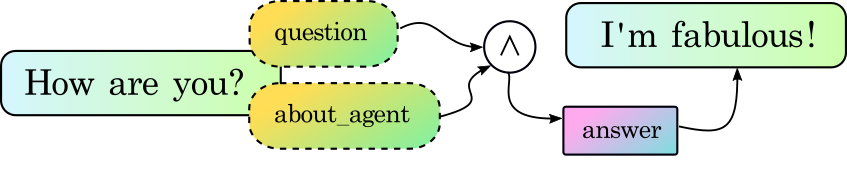
\includegraphics[scale=0.7]{figs/ex1.png}
\captionof{figure}{Example of a causal signal-state production relationship.}
\label{fig:ex1}
\end{Figure}

Such combinations of signals are modelled as \textbf{Conditions} in \rasta:

\begin{definition}[Condition]
The condition set $\mathsc{Cond}(C)$ is a boolean algebra over signals $C$: Let $\mathsc{Cond}(C) := \mathsc{Cond}(C \cup \bigcup_{(c_x, c_y) \in C \times C}{\{c_x \land c_y, c_x \lor c_y\}})$. The definition of the $\mathsc{Eval}$ function for conditions is extended as follows: 
\end{definition}

In \rasta, productions are directly adapted into a generic state machine: 

\begin{definition}[Property-Changed-Signal]
\end{definition}

\begin{definition}[State]
A state $T^i$ is a six-tuple $\langle P^i_R \subset P, P^i_W \subset P, \mathsc{on}^i \in \mathsc{Cond}, f^i : P_R, P_W \rightarrow \mathsc{Result}, C^i_\text{emit} \subset C \rangle$: It can write to a set of properties $P^i_W$, read from a set of properties $P^i_R$, execute it's state function $f^i$ in reaction to the condition $\text{\textsc{on}}^i$, and emit spikes for a subset of signals $C^i_\text{emit}$. 
\end{definition}

The input question \textit{How are you} is held by a \textbf{Property} $p_1 \in P$. For the given example, the \textsc{question} and \textsc{about\_agent} events are \textbf{Signals} $\{c_1, c_2\} \subset C$ out of a superset of signals C. In order to close the gap between the property $p_1$ and it's derivative signals, an intermediate signal is introduced: As $p_1$ adapts a new value, it emits a \textsc{changed} signal $c_0 \in C$. Furthermore, note the following definition of a \textbf{State} in \rasta:

The \textsc{answer} state is a \textbf{State} $t_1 \in T$.  \\

% Instances of these signals are the \textbf{Spikes} $\{\hat{s_{c_1}} and \hat{s_{c_2}}\} \subset \hat{S}$. The actual activation of the state $t_1$ is represented by a separate \textbf{Activation} object $a_1 \in A$, which is "consumed" once it runs.

The combination of States $T$, Activations $A$, Signals $C$, Spikes $\hat{S}$ and Properties $P$ is called a \textbf{Context} $H = \{T,A,C,\hat{S},P\}$.\\

\begin{Figure}
\centering
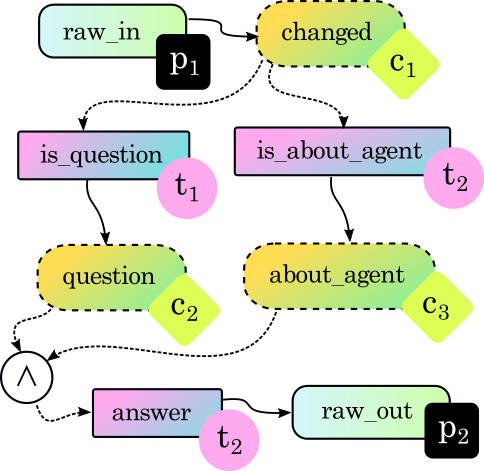
\includegraphics{figs/gra1.png}
\captionof{figure}{Signal-Flow Diagram for previous example.}
\label{fig:gra1}
\end{Figure}

\subsection{Signal Flow}

\textbf{States} $t \in T$ (Processes, Transition Functions, Transducers, Non-Terminals)\\

\textbf{Properties} $p \in P$  (Data, Channels)\\

\textbf{Signals} $c \in C$ (Constraints, Chunks)\\

\textbf{Spikes} $\hat{s_c} \in \hat{S}$\\

\textbf{Activations} $\hat{a_t} \in \hat{A}$\\

\textbf{CausalGroup spike equivalence classes} $[\hat{s_c}]$.\\

\subsection{The Transduction Operation}

\section{Conflict Resolution}

\subsection{Bayesian Specificity As State Utility}

\subsection{Causal Groups and Constraint Completion}

\subsection{Primary and Secondary Signals}

\section{Experiments}


\section{Conclusion}


\section{Future Work}


\section{References}


\end{multicols}
\end{document}
